\documentclass[loesung]{schulein}
%
\input{"/Volumes/Chris Nifty/01 Schule/01 Unterrichtsmaterial/TEMPLATES/ab_preamble"}
%
\usepackage{floatflt}
\usetikzlibrary{decorations.pathreplacing}

\kopfDatum{\today} 
\fach{in-z2}
\dokName{Array (Feld)}
\keineSeitenzahlen
%
\begin{document} 
\section*{Datenstruktur Array (Feld)}

\begin{floatingfigure}[r]{3.2cm}
%\vspace*{-.4cm}
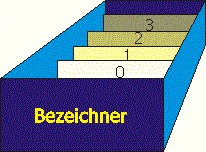
\includegraphics[width=3cm]{schachtel-array}
\end{floatingfigure}
%\textbf{Anschauliche Erklärung:} 
\textit{Arrays} (dt.: \textit{Felder}) sind spezielle Variablen, die mehr als einen Wert speichern können. Ein Array kann man sich wie eine Variable als Schachtel vorstellen. Allerdings hat diese Schachtel - im Gegensatz zu der einer einfachen Variablen - durchnummerierte Unterteilungen, in denen die Werte der einzelnen Elemente gespeichert werden.

Auf technischer Ebene ist ein Array eine Aneinanderreihung von Elementen eines festen Datentyps ($T$) im Speicher. Ein Zugriff auf die einzelnen Elemente wird über einen Index ($i$) möglich (vgl. Abb. \ref{fig_1}). Die Nummerierung beginnt mit 0.


%Die Adresse der $i$-ten Komponente lässt sich wie folgt berechnen
%\begin{align*}
%a_0+(i-1)\cdot size(T_0)
%\end{align*}

%\subsubsection*{Technische Umsetzung}
%Arrays werden im Speicher als Aneinanderreihung der Repräsentationen des Grundtyps dargestellt. Auf diese Weise entsteht für ein Array des Typs $T$ zum Grundtyp $T_0$, dessen erstes Element an der Adresse $a_0$ abgelegt wird, die in Abbildung 1 gezeigte Speicherrepräsentation, wobei $R(T_0)$ die Repräsentation eines Elementes des Grunddatentyps ist und $R(T)$ die des gesamten Arrays.

\begin{figure}[h]
\centering
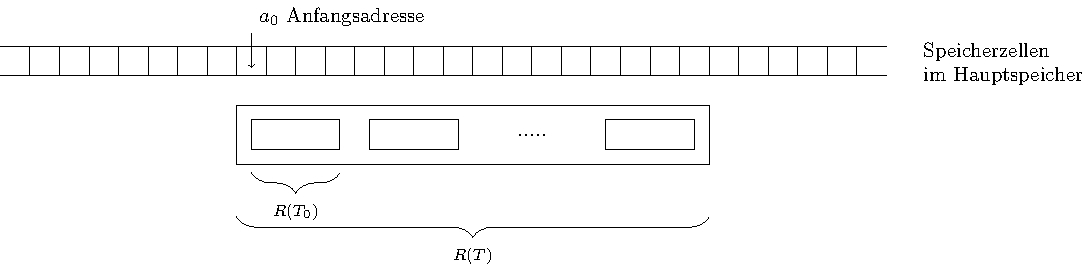
\includegraphics[scale=.8]{figure_1}
\caption{Speicherrepräsentation von Arrays}
\label{fig_1}
\end{figure}

\subsection*{Eigenschaften von Arrays}
\begin{smallitemize}
\item Arrays haben eine feste Größe (Anzahl von Elementen), die nach der Initialisierung nicht mehr verändert werden kann.
\item Die Elemente eines Arrays müssen alle denselben Datentyp aufweisen.
\end{smallitemize}

\subsection*{Arrays in Python}
Python stellt von Hause aus keine Implementierung von Arrays zur Verfügung. Sie können aber durch die viel mächtigere eingebaute Datenstruktur \textit{List} (dt.: Listen) realisiert werden. Listen implementieren noch viele Zusatzfunktionen, auf die wir hier aber nicht näher eingehen.

\Ueberschrift{Arbeitsauftrag}{task}
\begin{aufgaben}
\item \leicht Erklären Sie in maximal zwei Sätzen, was ein Array ist.
\item \mittel Erklären Sie mit Hilfe der Abbildung \ref{fig_1} wie die Werte eines Arrays im Speicher organisiert sind. Erläutern Sie zusätzlich die Formel $a_0+i\cdot size(T_0)$. Was lässt sich so berechnen? 
\item \schwer Begründen Sie, warum Arrays nur Elemente des gleichen Datentypen enthalten. %Schreiben sie einen kurzen Text.
\end{aufgaben}



\end{document}